%
\section*{Developing}%
%
\begin{frame}%
\frametitle{Software Development Process}%
\begin{itemize}%
\item In the \optimizationBenchmarking\ project, we follow a distributed, concurrent software development process%
\item<2-> We use \git\expandafter\scitep{\gitReferences} as versioning system\uncover<3->{ and \gitHub\expandafter\scitep{\gitHubReferences} for hosting}%
\item<4-> For building and dependency management, we use \maven%
\item<5-> As developer environment, we recomment \eclipse\expandafter\scitep{\eclipseReferences} (version $\geq$ Luna), as it natively supports \git\ and \maven\expandafter\scitep{\mavenReferences}.%
\end{itemize}%
\end{frame}%
%
\begin{frame}[t]%
\frametitle{Contribution Lifecycle}%
\begin{enumerate}%
\item Prerequisites\only<2-4>{:%
\begin{enumerate}%
\item Obtain a \gitHub\ account%
\item<3-> Register a public/private key pair for your account%
\item<4-> Join group \expandafter\href{\optimizationBenchmarkingURL}{\texttt{optimizationBenchmarking}}%
\end{enumerate}}%
%
\item<5-> Fork project\only<-5>{ \expandafter\href{\optimizationBenchmarkingURL}{\texttt{optimizationBenchmarking/optimizationBenchmarking}}}%
\item<6-> Add your code\only<-6>{, e.g., an own evaluation module, in the appropriate location (maybe an own package)}%
\item<7-> Test your code\only<8-9>{%
\begin{itemize}%
\item add \junit\expandafter\scitep{\junitReferences} tests if possible%
\item<9-> provide examples, example data, and expected results%
\end{itemize}%
}%
\item<10-> Make sure your code is properly documented\only<-10>{ and that your commits contain sufficient explanations}%
\item<11-> Create a \texttt{pull request}\only<-11>{, i.e., ask me to include your code in the main project}%
\item<12-> After a discussion, your code will (very likely) become part of the main project%
\end{enumerate}%
%
\end{frame}%
%
%
\begin{frame}%
\frametitle{Import Fork into Eclipse}%
%
\only<-4>{%
\begin{itemize}%
\item Importing a project (or fork) from \gitHub\ into \eclipse\ means to clone it to a local repository and then to work on that repository.%
\item<2-> Although \gitHub\ offers cloning via HTTPS as the default, for me it worked better with SSH.%
\item<3-> After cloning and importing the clone into \eclipse, you need to update the project with \maven\ to properly initialize the project structure and dependencies.%
\item<4-> In the following, I provide a step-by-step screenshot series on how to do all of that\dots%
\end{itemize}%
}%
%
\locate{5}{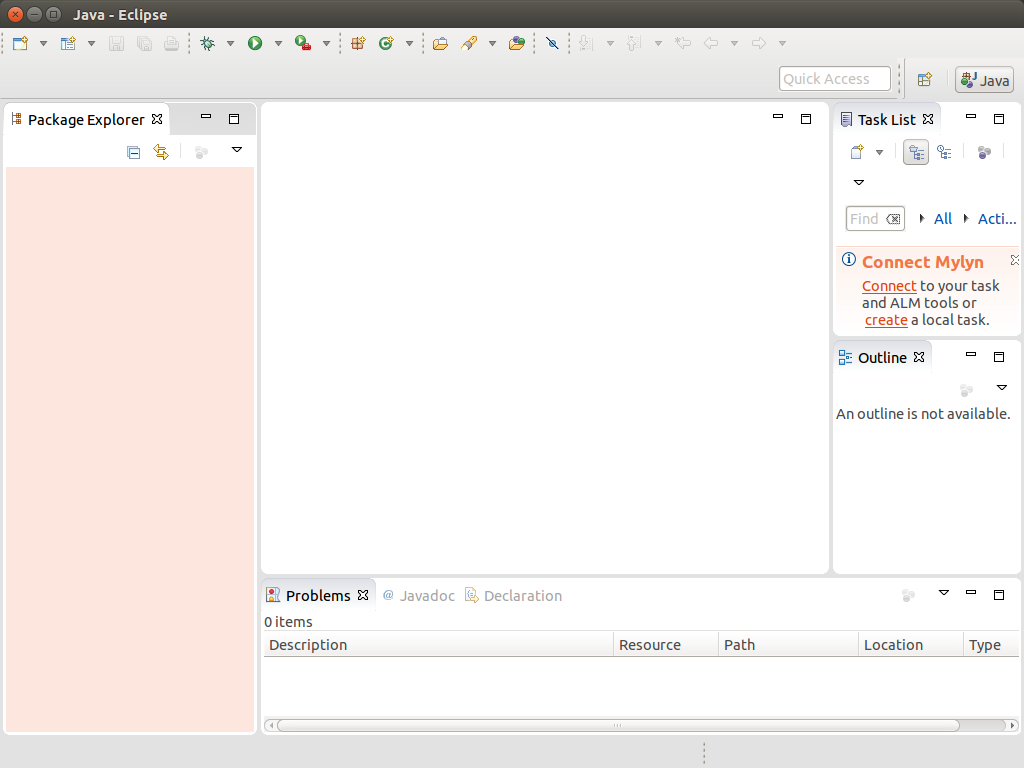
\includegraphics[width=0.75\paperwidth]{\sharedPath/graphics/developing/import_git_project_into_eclipse/annotated/import_git_project_into_eclipse_01}}{0.125}{0.16}%
%
\locate{6}{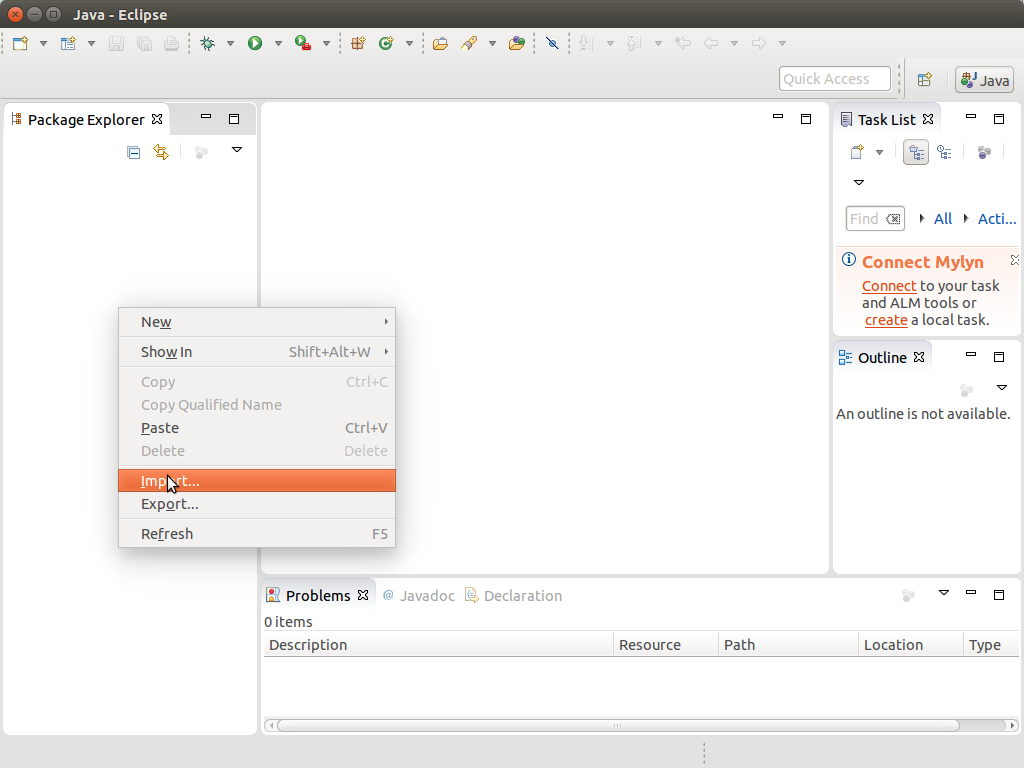
\includegraphics[width=0.75\paperwidth]{\sharedPath/graphics/developing/import_git_project_into_eclipse/annotated/import_git_project_into_eclipse_02}}{0.125}{0.16}%
%
\locate{7}{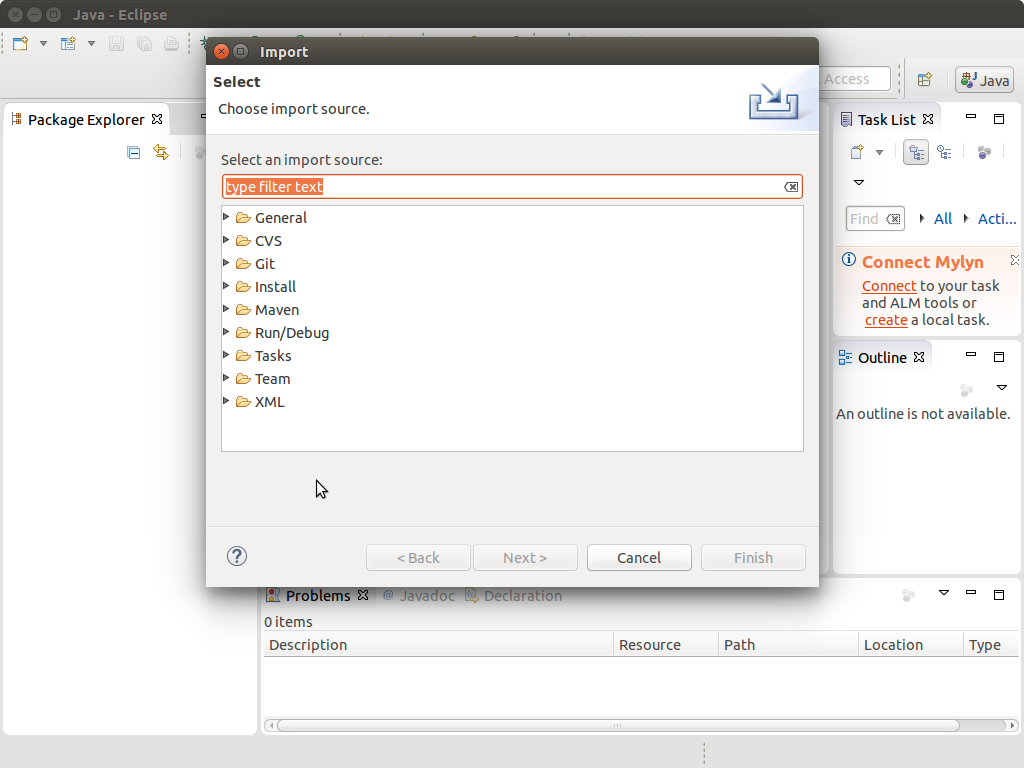
\includegraphics[width=0.75\paperwidth]{\sharedPath/graphics/developing/import_git_project_into_eclipse/annotated/import_git_project_into_eclipse_03}}{0.125}{0.16}%
%
\locate{8}{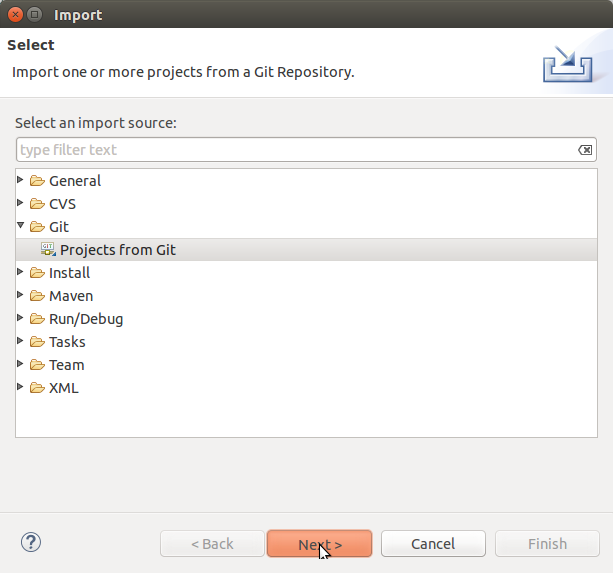
\includegraphics[width=0.625\paperwidth]{\sharedPath/graphics/developing/import_git_project_into_eclipse/annotated/import_git_project_into_eclipse_04}}{0.1875}{0.15}%
%
\locate{9}{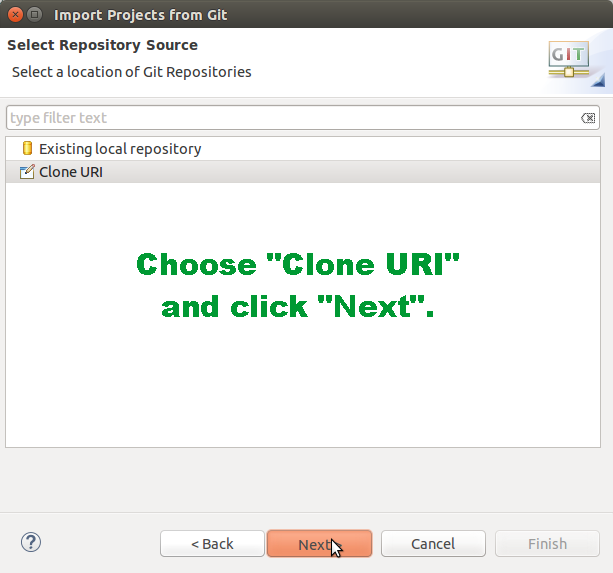
\includegraphics[width=0.625\paperwidth]{\sharedPath/graphics/developing/import_git_project_into_eclipse/annotated/import_git_project_into_eclipse_05}}{0.1875}{0.15}%
%
\locate{10}{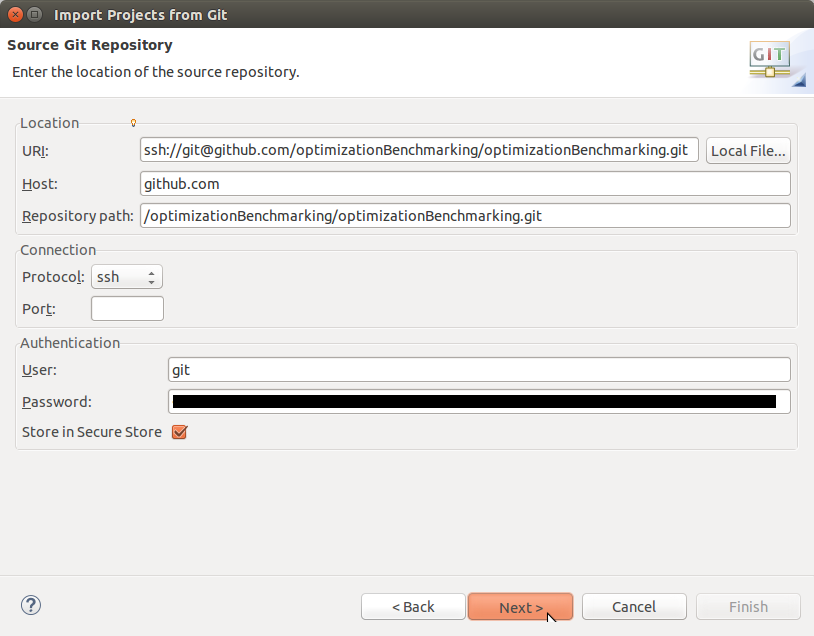
\includegraphics[width=0.73\paperwidth]{\sharedPath/graphics/developing/import_git_project_into_eclipse/annotated/import_git_project_into_eclipse_06}}{0.15}{0.145}%
%
\locate{11}{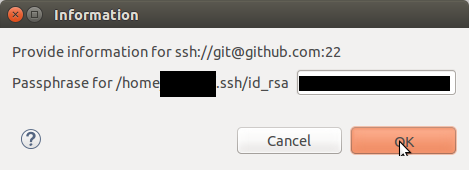
\includegraphics[width=0.8\paperwidth]{\sharedPath/graphics/developing/import_git_project_into_eclipse/annotated/import_git_project_into_eclipse_07}}{0.1}{0.18}%
%
\locate{12}{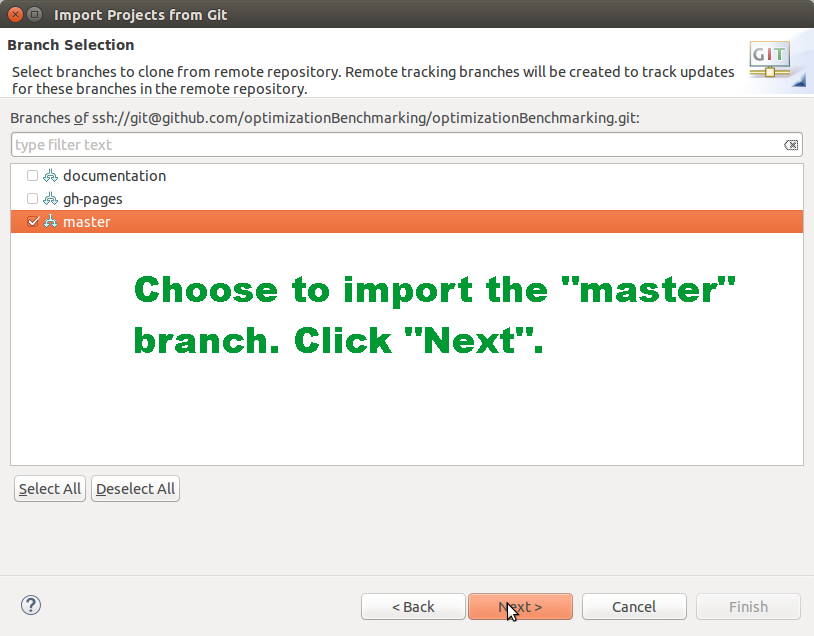
\includegraphics[width=0.75\paperwidth]{\sharedPath/graphics/developing/import_git_project_into_eclipse/annotated/import_git_project_into_eclipse_08}}{0.125}{0.15}%
%
\locate{13}{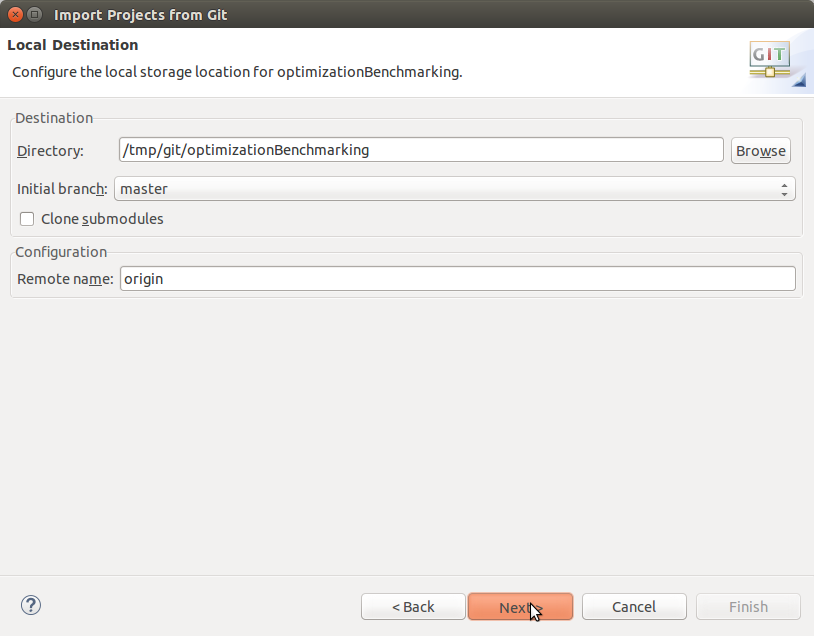
\includegraphics[width=0.75\paperwidth]{\sharedPath/graphics/developing/import_git_project_into_eclipse/annotated/import_git_project_into_eclipse_09}}{0.125}{0.15}%
%
\locate{14}{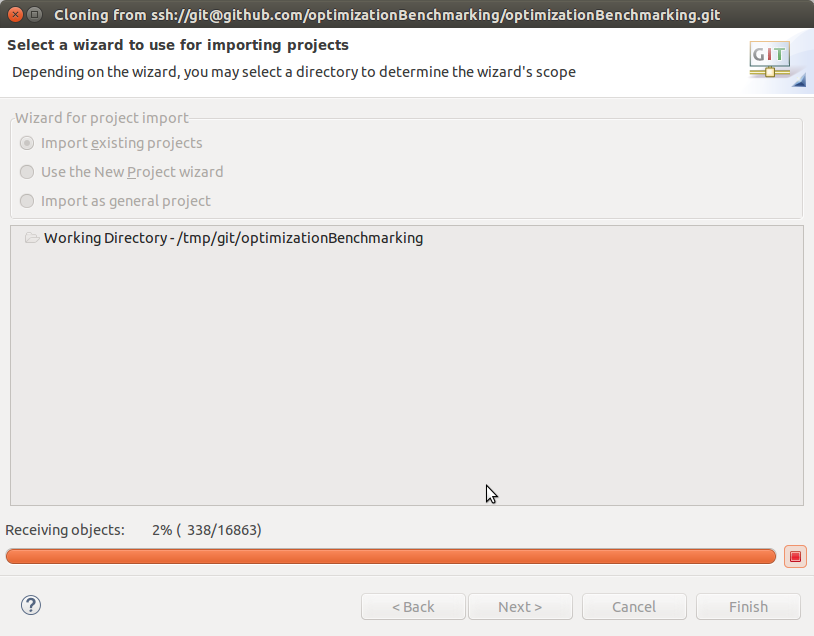
\includegraphics[width=0.75\paperwidth]{\sharedPath/graphics/developing/import_git_project_into_eclipse/annotated/import_git_project_into_eclipse_10}}{0.125}{0.15}%
%
\locate{15}{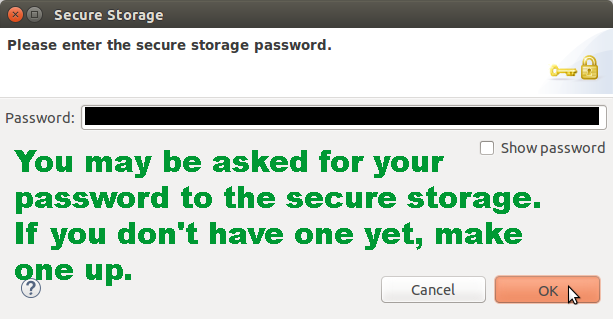
\includegraphics[width=0.9\paperwidth]{\sharedPath/graphics/developing/import_git_project_into_eclipse/annotated/import_git_project_into_eclipse_11}}{0.05}{0.185}%
%
\locate{16}{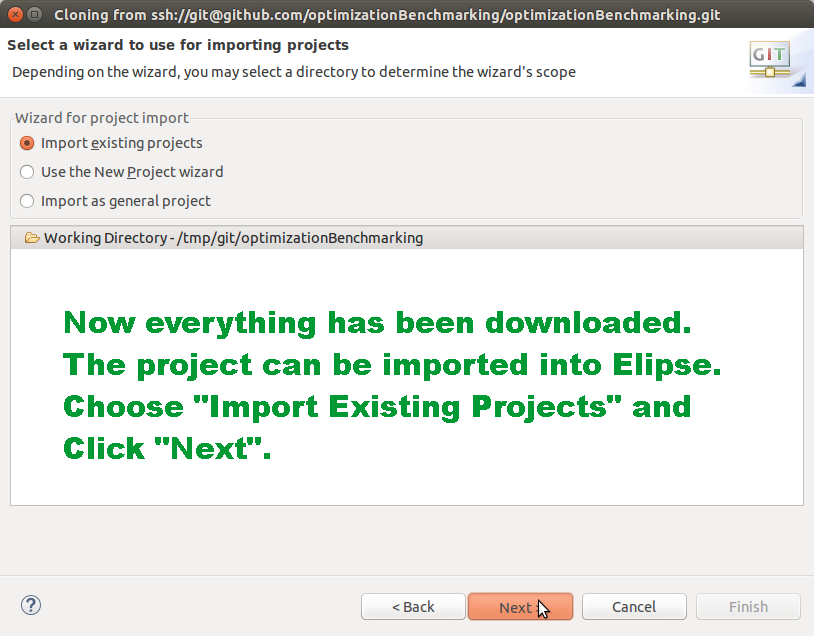
\includegraphics[width=0.75\paperwidth]{\sharedPath/graphics/developing/import_git_project_into_eclipse/annotated/import_git_project_into_eclipse_12}}{0.125}{0.15}%
%
\locate{17}{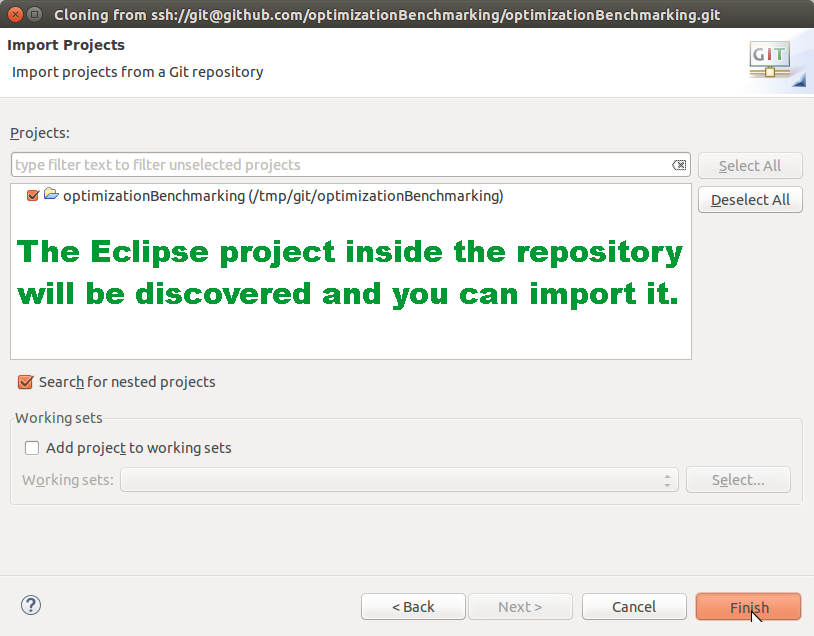
\includegraphics[width=0.75\paperwidth]{\sharedPath/graphics/developing/import_git_project_into_eclipse/annotated/import_git_project_into_eclipse_13}}{0.125}{0.15}%
%
\locate{18}{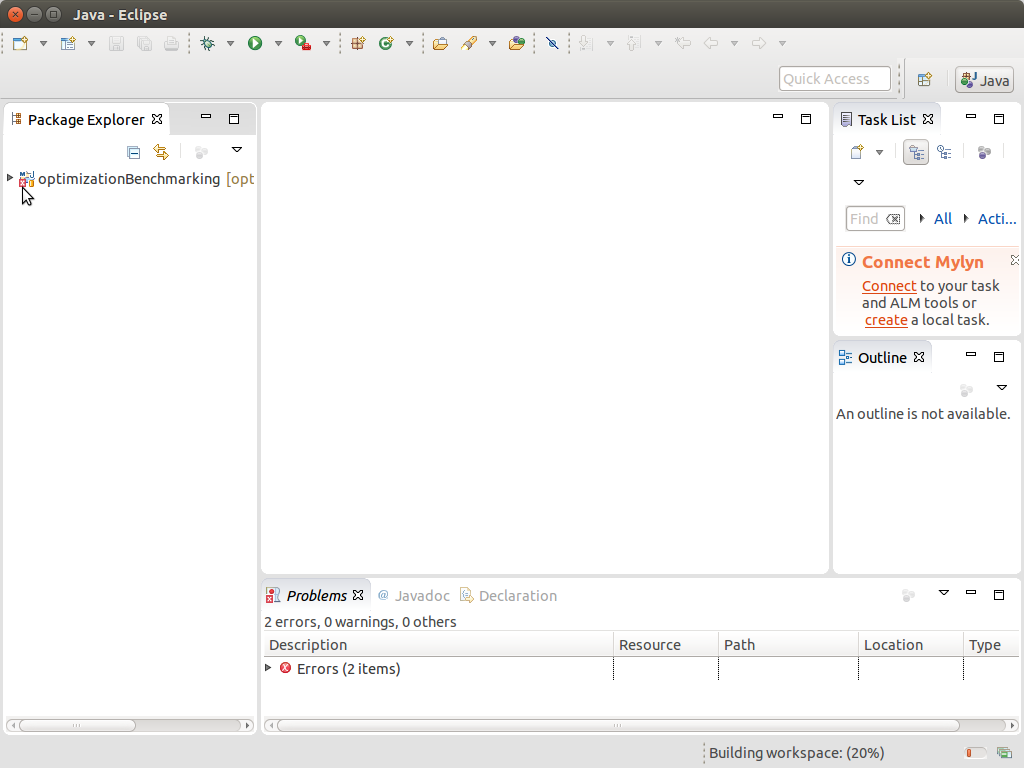
\includegraphics[width=0.8\paperwidth]{\sharedPath/graphics/developing/import_git_project_into_eclipse/annotated/import_git_project_into_eclipse_14}}{0.1}{0.145}%
%
\locate{19}{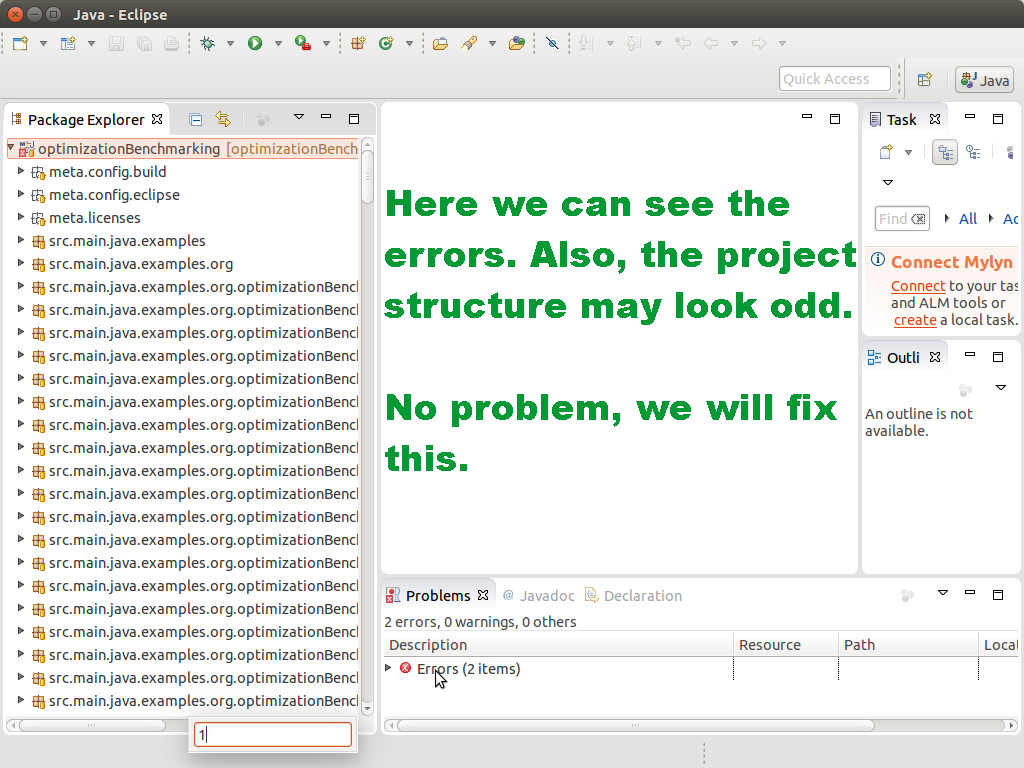
\includegraphics[width=0.8\paperwidth]{\sharedPath/graphics/developing/import_git_project_into_eclipse/annotated/import_git_project_into_eclipse_15}}{0.1}{0.145}%
%
\locate{20}{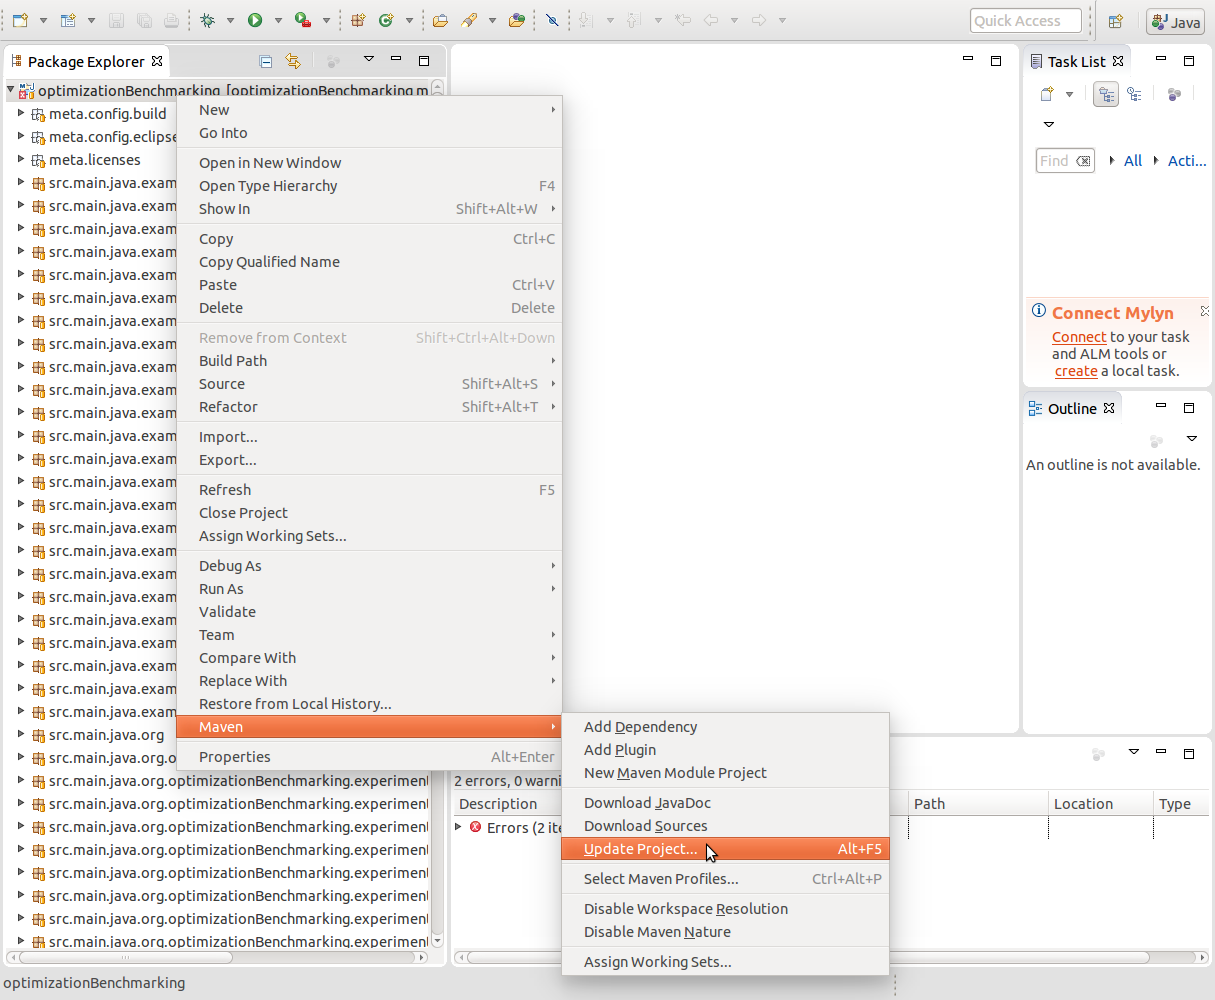
\includegraphics[width=0.7\paperwidth]{\sharedPath/graphics/developing/import_git_project_into_eclipse/annotated/import_git_project_into_eclipse_16}}{0.15}{0.15}%
%
\locate{21}{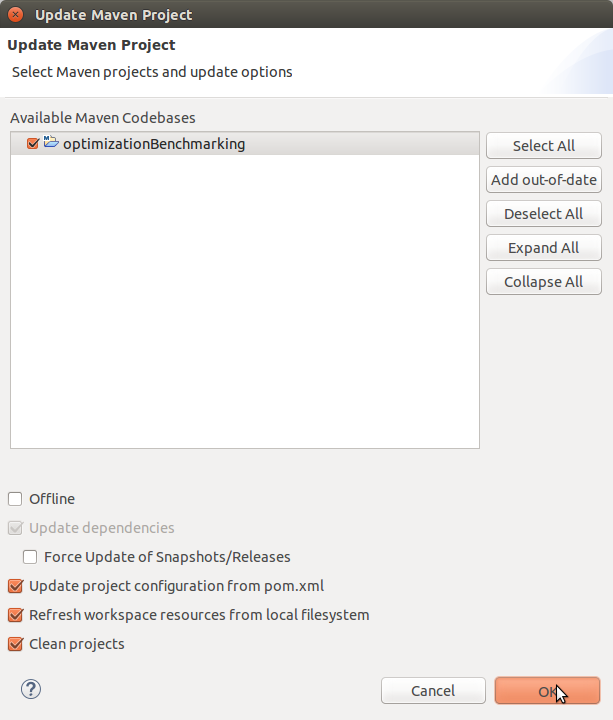
\includegraphics[width=0.5\paperwidth]{\sharedPath/graphics/developing/import_git_project_into_eclipse/annotated/import_git_project_into_eclipse_17}}{0.25}{0.1525}%
%
\locate{22}{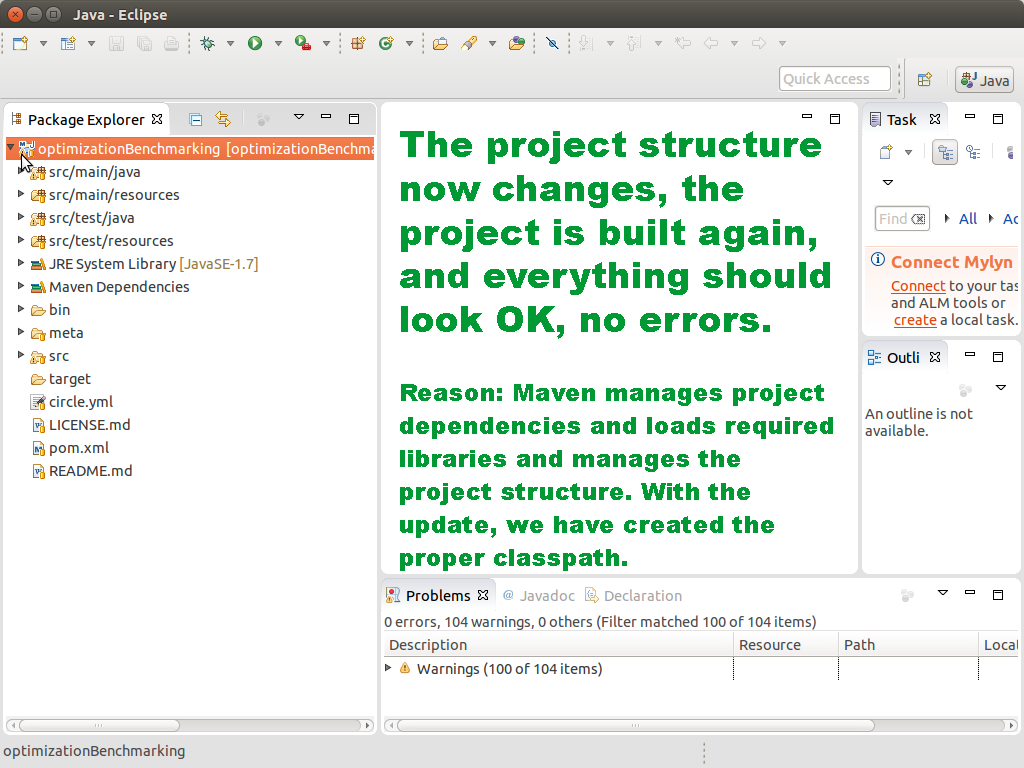
\includegraphics[width=0.8\paperwidth]{\sharedPath/graphics/developing/import_git_project_into_eclipse/annotated/import_git_project_into_eclipse_18}}{0.1}{0.1425}%
%
\end{frame}%
%